\documentclass[12pt, letterpaper]{article}
\usepackage{times}
\usepackage{graphicx}
\usepackage{import}
\usepackage{fancyhdr}
\usepackage{wrapfig}
\usepackage[utf8]{inputenc}
\usepackage[hidelinks]{hyperref}
\usepackage{subcaption}
\usepackage{pdfpages}
\pagestyle{fancyplain}% <- use fancyplain instead fancy
\fancyhf{}
\addtolength{\headheight}{15pt}
\fancyhead[L]{Cyber Security - Konstantinos Poumpouridis}% <- added
\fancyhead[R]{488394}
\fancyfoot[C]{\thepage}
%\renewcommand\headrulewidth{0pt}% default ist .4pt
\renewcommand{\plainheadrulewidth}{.4pt}% default is 0pt
\title{Semester 4: Body of Knowledge}
\author{Konstantinos Poumpouridis}
\date{08/02/2023}
\pagenumbering{arabic}
\begin{document}
\maketitle
\thispagestyle{empty}
    
\newpage
\section{Changelog}
    \begin{table}[htbp]
        \begin{tabular}{|l|l|l|}
            \hline
            Version & Changes         & Date   \tabularnewline \hline
            0.1     & Added BOK week (1-4) & 08/02/23 \tabularnewline \hline
        0.2  &  Added week 1 + Attachment 1 & 14/02/23 \tabularnewline \hline
       0.2.1     &    Added notes for week 2, Attachment notes reworked     &  16/02/23      \tabularnewline \hline
       0.2.2  &  Finished week 2 + reworked attachment in Attachment 1 & 18/02/23 \tabularnewline \hline
       0.2.3  &  Finished 1st advanced task  & 26/02/23 \tabularnewline \hline
       0.3  &  Finished week 3  & 03/03/23 \tabularnewline \hline
        0.3.1  &  Finished week 5  & 21/03/23 \tabularnewline \hline
        0.3.2  &  Finished roughly finished week 4  & 28/03/23 \tabularnewline \hline
        \end{tabular}
    \end{table}
\newpage
\tableofcontents
\newpage
\section{Introduction}
\begin{wrapfigure}{1}{0.25\textwidth}
    \includegraphics[width=0.25\textwidth]{fotos/Kosta.jpeg}
    \caption{Picture of me}
\end{wrapfigure}
My name is Konstantinos Poumpouridis or in short Kosta. I was born in 11 June 1999 in Thessaloniki.

\subsection{My background}

What I do in my spare time is working on open-source projects and tinker with computers. My recent projects are making everything accessible with my iPad Pro like working with Windows 365 or with vCenter or code through Github code space. I also do fitness and sim racing.
\hfill\break
\\
I also have a LinkedIn page where you can see how many certificates I've achieved.
\hfill\break
\url{https://www.linkedin.com/in/konstantinos-poumpouridis-552080171/}
\\
\newpage
\subsection{My hobby's}

\subsubsection{Sim-racing}
%Yes, an expensive hobby to have but my love for motorsport is huge.  It started with Rally since that rally is big in Greece (due to all the rocky roads hahaha) eventually I went to go on Gran Turismo 4 and fell in love. My family gifted me a steering wheel and that's when I knew that I love cars and racing. Now I follow WRC, Le Mans, Formula 1 and IMSA.
Having a love for motorsport is indeed a costly hobby, but my passion for it is immense. It all began with Rally, which is quite popular in Greece due to the abundance of rocky roads. From there, I discovered Gran Turismo 4 and became enamored with it. The gift of a steering wheel from my family solidified my love for cars and racing, and now I avidly follow events such as WRC, Le Mans, Formula 1, and IMSA.
\begin{center}
    \includegraphics[width=0.8\textwidth]{fotos/simracingkosta.jpeg}
\end{center}
I began playing in 2021 and earned a few trophies along the way. While I don't play as frequently as I would like, this is partly due to my broken steering wheel and the costly monthly subscription fee of \$13.


\newpage
\section{Web Application Security (week 1-4)}
\subsection{Week 1}
%In the beginning, we were slowly discovering some tools to use. We started first installing Kali Linux in vCenter and a Ubuntu server for Juice shop and DWVA for other testing software. There also was a workshop on Friday (10 Oct) which I attended. There were 2 workshops, One was about introduction to Infrastructure which I skipped and the second one was about hacking-related coding basic but I followed this one. 
At the start, we gradually learned about various tools and their uses. Our initial steps included installing Kali Linux in vCenter, Ubuntu server for Juice Shop, and DWVA for other testing purposes. On Friday, October 10th, there was a workshop which I attended. Out of the two workshops scheduled, I chose to attend the second one, which focused on basic coding in relation to hacking, while I skipped the first one, which was an introduction to Infrastructure.
\break
\\
%The workshop that I attended was from Tom Broumels and he was explaining how simple it is to inject code if no line checks if the request is not something malicious. I made some quick notes while he was presenting. you can see it in "Attachment 1: Workshop hacking related coding basic notes" or you can press this hyperlink down here.
I recently attended a workshop led by Tom Broumels, where he demonstrated how easy it is to inject code when proper checks are not in place to prevent malicious requests. During the workshop, I took some notes, which can be viewed in "Attachment 1: Workshop hacking related coding basic notes". Alternatively, you can access the notes by clicking on the hyperlink below.
\hyperref[workshop:week1]{\textbf{Press here to see my notes from the workshop!}}

\newpage
\subsubsection{Set-up of a test Web Shop}

\begin{figure}[!ht]
    \centering
    \begin{subfigure}{.5\textwidth}
        \centering
        \includegraphics[width=.8\linewidth]{fotos/Bok week 1/Week_1_install_vmware.jpeg}
        \caption{My VM's on my vCenter}
%        \label{fig:sub1}
    \end{subfigure}%
    \begin{subfigure}{.5\textwidth}
        \centering
        \includegraphics[width=.8\linewidth]{fotos/Bok week 1/Pfsense_install.jpeg}
        \caption{PFSense configured}
%        \label{fig:sub2}
    \end{subfigure}
    \begin{subfigure}{.5\textwidth}
    \centering
    \includegraphics[width=.8\linewidth]{fotos/Bok week 1/Juice shop installed.jpeg}
    \caption{Juice shop pulled and ready to be installed}
    \label{fig:sub3}
\end{subfigure}%
%\begin{subfigure}{.5\textwidth}
%    \centering
%    \includegraphics[width=.8\linewidth]{fotos/Kosta.jpeg}
%    \caption{Place holder}
%    \label{fig:sub4}
%\end{subfigure}
\end{figure}\mbox{}\\
\hfill
\\
On the second day of our school, we went on to install some virtual machines into our vCenter. We had to install Kali Linux (of course) since that will be our main operating system to use hack tools this semester. second but optional is to install PFSense so that other students don't go to our systems and destroy anything in it. and the last one was to install Juice Shop and or DVWA which are two testing environment for pen testing.
\newpage
\subsubsection{Threat + Risk Analysis for the test Web Shop}

Risk Analysis: (optional if other CIA and Risk Matrix assignments are done)

\includegraphics[width=1.1\textwidth]{fotos/Bok week 1/Riskanalysis.jpeg}
\break
Business Continuity: 
\hfill\break
\includegraphics[width=1.1\textwidth]{fotos/Bok week 1/Riskanalysis2.jpeg}
\break
*rest damage is an estimate of the damage that can be done after the measurement is implemented, your risk will never be 0.0 and no assurance can be given at any time.
\break
\newpage
\begin{enumerate}
    \item \textbf{Burglar:} The security measures I choose against Burglars are Security cameras, Security Personal and Key card authentication. The security cameras and security personnel speak for themselves with these 2 measurements you reduce criminals who want to break in and Key cards make it a lot harder for your criminals.
    \item \textbf{Virus:} Viruses come in different forms and shapes and worse keep evolving just like a real virus does to our immune system. Good thing that Antivirus exist which helps us detect viruses and contain them. But the best virus scanner is your brain and what I mean by it is when you see a shady link or a file that you don't click it straight away and think about it if it's safe or not. That's why people need virus awareness training so they don't get viruses in their systems.
    \item \textbf{Trojan/Phishing:} Trojans and phishing are meant to infiltrate your systems and steal and or ransom your data. Most of the Phishing and Trojans come from emails disguised as the government or some company. So my solution for this has some monitoring tools for your mail and some intelligent filter to keep out spam and unwanted mail coming to your mail servers. Plus you can also train your employees in some Phishing and Trojan awareness training.
    \item \textbf{Short circuit:} A short circuit happens randomly and the best solution is to have a fire extinguisher and to keep your hardware maintained at all times to reduce the chances of a short circuit. Of course, there is enterprise hardware which ensures longer durability and also has longer warranty to make sure that you get what you got promised.
    \item \textbf{Fire:} Fire is unpredictable so it is better to be prepared if it is happing. Fire can come from many reasons from overheating to short circuits, so these 3 things are mandatory in my opinion. The first one is Fire extinguishers because first of all, it is mandatory to have one in the office and second it is a solid solution and is not dangerous compared to carbon dioxide extinguisher which is dangerous because if someone gets stuck in the server room they can suffocate in the room due to lack of oxygen
    \item \textbf{Power outage:} Power outages not only go your servers go offline but your whole office building goes out of electricity as well. That's why I recommend installing UPS and a generator. Let's start with UPS or an Uninterruptible Power Supply it's meant once the electricity goes down that you have enough time to safely shut down your servers. A generator is mostly used after the disaster so that you have some electricity but the problem with generators is that they take time to startup which is a problem when you need to prevent your servers from sudden outages.
\end{enumerate}

\subsubsection{Coding for hackers part 1: Web Programming}
Go to Attachment 1 for more information.
\\
\hyperref[workshop:week1]{\textbf{My notes about this workshop is in Attachment 1}}
\newpage
\subsubsection{Basic Hacking and Pentesting Proces}
\emph{You should be able to explain in your BoK:}
\begin{itemize}
    \item \emph{What are the process steps of every pentest in general?}
    \item \emph{What are the minimal requirements for a good pentest contract and pentest report?}
\end{itemize}

\textbf{What are the process steps of every pentest in general?}
\hfill\break
The first step for pen testing is of course to gather some information or "Intel Gathering" because before you want to know some company information like phone numbers, names and emails. Once the hacker has all the information that it needs. The second step is to plan out your idea before you attack. What I mean by it is to get an idea of what ports may be open or which range they would use this is called footprinting.
\hfill\break
\\
\emph{"Footprinting (also known as reconnaissance) is the technique used for gathering information about computer systems and the entities they belong to. To get this information, a hacker might use various tools and technologies. This information is very useful to a hacker who is trying to crack a whole system." - Wikipedia contributors. (2023, 18 januari). Footprinting. Wikipedia. Geraadpleegd op 14 februari 2023, van https://en.wikipedia.org/wiki/Footprinting}
\hfill\break
Now the third step checking for any vulnerabilities this is when you go in-depth into your pen testing. You'll be using these tools to find any exploits:
\begin{itemize}
    \item Tooling: web application proxies \& web browser
    \item XSS and CSRF
    \item SQL Injection
    \item Path Traversal
    \item Network Sniffing and Spoofing
\end{itemize}
\hfill\break
\newpage

Lets start with \textbf{Tooling: web application proxies \& web browser}
\hfill\break
\\
In most browsers, there is a program called "Dev Tools" which you can inspect the page in code. There are also external applications for web proxies like Burp Suite or OWASP ZAP.
\hfill\break
\hfill\break

\textbf{XSS and CSRF}
\hfill\break
\hfill\break

\textbf{SQL Injection}
\hfill\break
\hfill\break


\textbf{Path Traversal}
\hfill\break



\textbf{Network Sniffing and Spoofing}
\hfill\break


This information has been sourced by: Basic Hacking and Pentesting Proces. (z.d.). FHICT. Geraadpleegd op 14 februari 2023, 
\hfill\break
van https://fhict.instructure.com/courses/12919/pages/reference-basic-hacking-and-pentesting-proces
\newpage
\subsubsection{DVWA: Command Injection}
After deploying my DVWA into my VCenter environment I started to log in to my DVWA website and changed the security to low for testing and learning. I started with low security to find out how to inject commands.
\hfill\break

\begin{figure}[!ht]
    \centering
    \begin{subfigure}{.5\textwidth}
        \centering
        \includegraphics[width=1\textwidth]{fotos/Bok week 1/DVWA/DVWA-login.png}
        \caption{DVWA login}
        \label{fig:sub6}
    \end{subfigure}%
    \begin{subfigure}{.5\textwidth}
        \centering
        \includegraphics[width=1\textwidth]{fotos/Bok week 1/DVWA/DVWA-settings-low.png}
        \caption{DVWA sececurity system}
        \label{fig:sub7}
    \end{subfigure}
\end{figure}\mbox{}\\
\hfill \break
Starting with code injection. Since that the server from DVWA does not checking. 
\newpage

\begin{figure}[!ht]
    \begin{subfigure}{.5\textwidth}
        \centering
        \includegraphics[width=1\textwidth]{fotos/Bok week 1/DVWA/Command-injection-tested-loitering-low.jpeg}
        \caption{Testing the code with uname -a}
        \label{fig:sub1}
    \end{subfigure}%
    \begin{subfigure}{.5\textwidth}
        \centering
        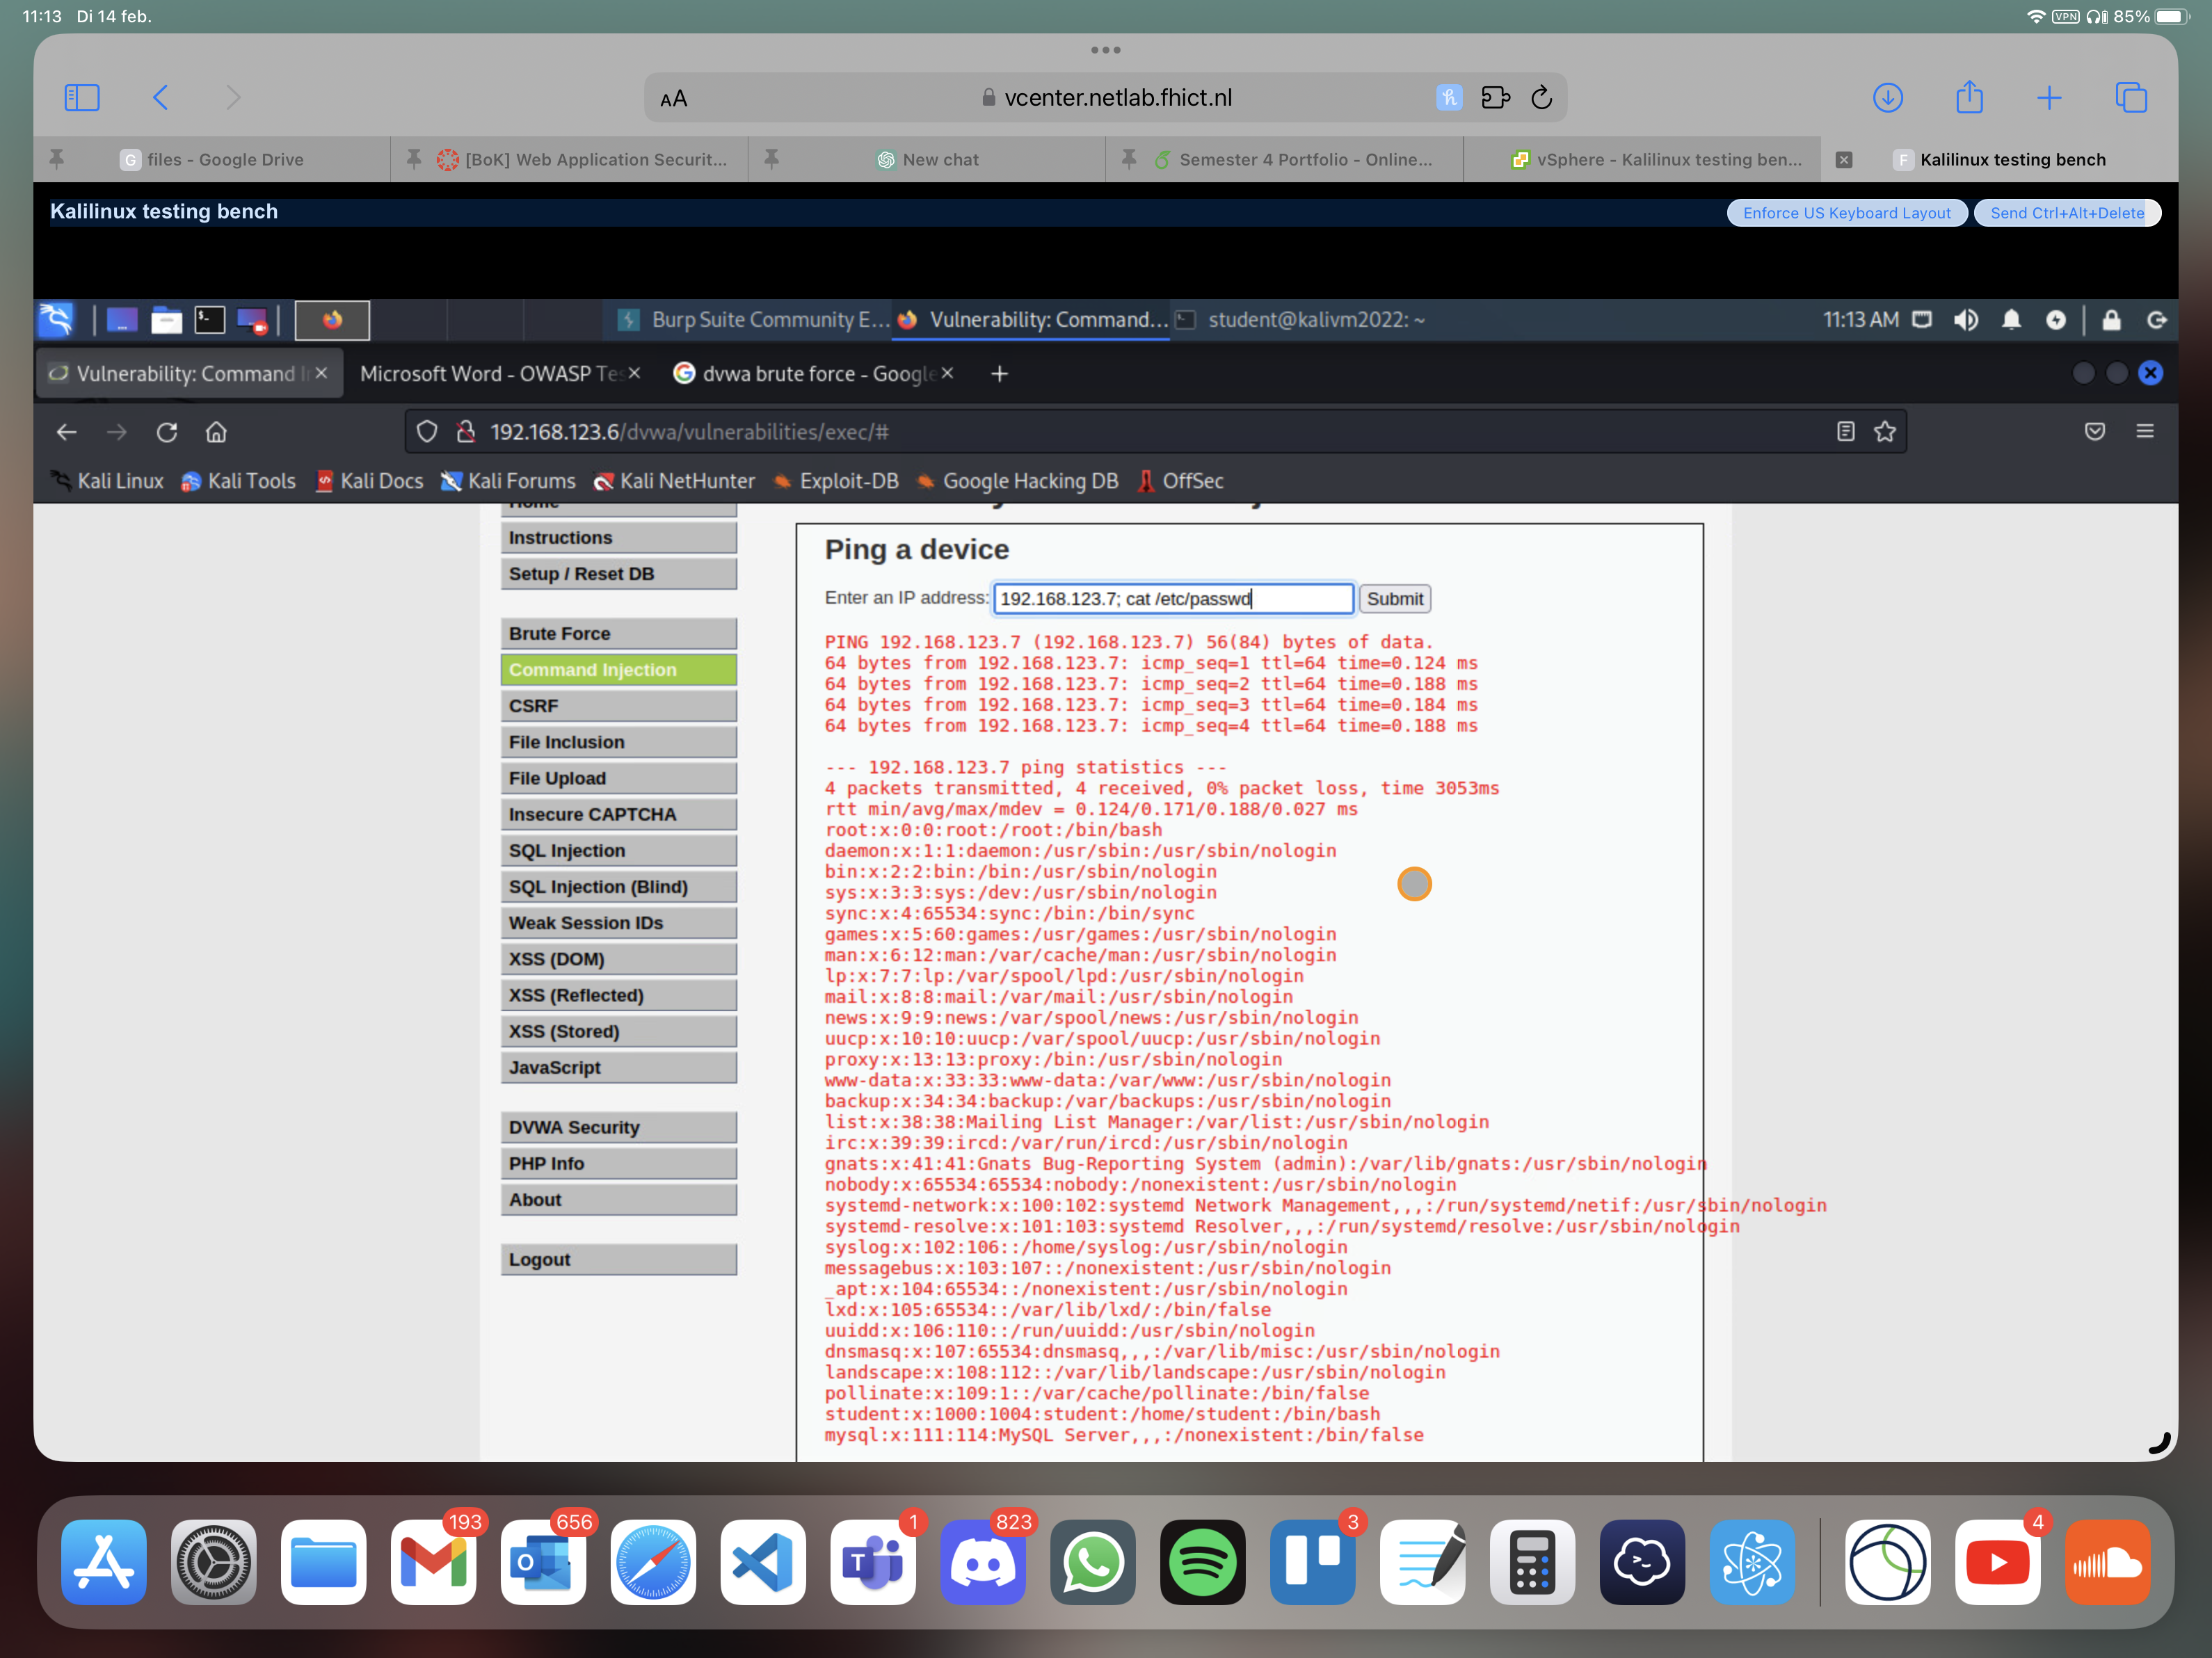
\includegraphics[width=1\textwidth]{fotos/Bok week 1/DVWA/Command-inject-passed-low.png}
        \caption{Testing the code with "IP; cat /etc/passwd"}
        \label{fig:sub2}
    \end{subfigure}
\end{figure}\mbox{}\\
\hfill\break
The low security does not check that my request I'm sending through the IP search bar which means I can send bash commands alongside the IP request.
\newpage
\subsection{Week 2}
\textbf{Wensday}
Today we had a workshop about First phase of hacking 
\hfill\break
\\
\hyperref[workshop:week2]{\textbf{Press here to see my notes from the workshop!}}
\hfill\break
\\
The teacher has showed the link to group project and pen test pre engagement. Still waiting for Floris to green lit or red lit it. Konstantin has a proposition but the problem. I made a proposition to make a pen testing in Vanderlande that they have an environment. We asked some questions about if we have to typing all of it and he responded that “if you have the time than do it but consider how much time you have”. So I’ve send my first draft to my teacher which wasn’t finished but now it is little more clear how we write our documents.
\hfill\break
\\
Note to the company:
We are ethical student we don’t want to destruct the environment.
\hfill\break
\\
\textbf{Our group agreement}
\hfill\break
\\
On the 15th of February, we assigned each other roles and then started to make the rules. We wanted to make sure that everyone agreed upon this rule.
\hfill\break 
\\
\textbf{Project leader:}
\hfill\break
The First role that we assigned was me, the group and my coach unanimously decided that I should be the project leader due to my load mouth.

\textbf{Note taker:}
\hfill\break
The second role was assigned also by me and Konstantin since no one wanted to take notes so I took it upon myself and Konstantin.

\textbf{Product owner:}
\hfill\break
Dean van Deijck is selected as a product owner. He has experience from his previous groups in how to manage and deliver the end product. So I and the group has faith in him that he will guide us to Proficient.

\textbf{Development team:}
\hfill\break
Konstantin, Petar and Floris are our development team which fills every part that we miss in our project.

\hfill\break
\hfill\break
\textbf{Workshop: lockpicking}
This Friday we had suppose to have Kuberneties workshop but that is changed to lock-picking. We had demo from Marco and he told us different tools for different lock 

\hyperref[workshop:week2Lockpicking]{\emph{Here is my notes for the lockpicking workshop}}
\newpage
\subsubsection{Footprinting, Reconnaissance and Social Engineering}
\textbf{The task}
\hfill\break
\includegraphics[width=1\textwidth]{PDFs/Week 2/Opdracht footprinting.jpeg}
\hfill\break
\textbf{Explain why this is an important phase of the pentesting proces.}
\hfill\break
In short, footprinting is a phase where you start gathering information about your target. Once you gathered enough information by finding addresses like mail, IP addresses, open ports, names and phone numbers Then your settle to pen test your target.

\hfill\break
\hfill\break
\textbf{ Make sure that you can show and explain at least 3 different techniques for searching useful information}
\hfill\break
\hfill\break
There are 3 different techniques that I used in this exercise
\begin{enumerate}
    \item The Harvester
    \item Maltego
    \item Lix - LinkedIn Scraping \& Email Finder
\end{enumerate}
\hfill\break
\hfill\break
The harvester:
\hfill\break
\hfill\break
\newpage
The Harvester or TheHarvester is a tool you can use to gather information from a domain. Once you entered your domain and which search engine you want to use. The tool will gather names, emails, IPs, subdomains and URLs.
\hfill\break
\hfill\break
I've tried it on my kali machine and these are my results.
\begin{figure}[!ht]
    \begin{subfigure}{0.45\textwidth}
        \centering
        \includegraphics[width=0.9\linewidth]{PDFs/Week 2/The harvester marktplaats tweakers.png}
        \caption{The harvester gathering info of Marktplaats and Tweakers}
    \end{subfigure}
    \begin{subfigure}{0.45\textwidth}
        \centering
        \includegraphics[width=0.9\linewidth]{PDFs/Week 2/Theharvest-fhict.png}
        \caption{The harvester gathering info of FHICT}
    \end{subfigure}
    \begin{subfigure}{0.45\textwidth}
        \centering
        \includegraphics[width=0.9\linewidth]{PDFs/Week 2/Theharvest-fontys.png}
        \caption{The harvester gathering info of Fontys}
    \end{subfigure}
    \begin{subfigure}{0.45\textwidth}
        \centering
        \includegraphics[width=0.9\linewidth]{PDFs/Week 2/Theharvester-vanderlande.png}
        \caption{The harvester gathering info of Vanderlande}
    \end{subfigure}
    \caption{My test on TheHarvester}
\end{figure}
I came across some colleagues on Vanderlande's website, which was unexpected. I was able to find Tim, who works in second-line support, and it was interesting to see.

\newpage
Maltego:
\hfill\break
\hfill\break
Acording to wiki:

\emph{Maltego is software used for open-source intelligence and forensics, developed by Paterva from Pretoria, South Africa. Maltego focuses on providing a library of transforms for discovery of data from open sources, and visualizing that information in a graph format, suitable for link analysis and data mining. As of 2019, the team of Maltego Technologies headquartered in Munich, Germany has taken responsibility for all global customer-facing operations.} - Wikipedia contributors. (2022, November 24). Maltego. Wikipedia. Retrieved February 19, 2023, from https://en.wikipedia.org/wiki/Maltego
\hfill\break
\hfill\break
In short Maltego is a data visualizer and analyzer tool which you can use to gather information about users, companies and networks in domains. It is used for information gathering to find vulnerabilities.
\hfill\break
\hfill\break
\textbf{Find how frontpage of nu.nl looked like 10 jears ago using waybackmachine.org}
\hfill\break
\hfill\break
\includegraphics[width=0.7\textwidth]{PDFs/Week 2/Wayback nu.png}
\hfill\break
\hfill\break
It wasn't hard to use it, All you need to do is paste the link https://ww.nu.nl/ and pick a date that you like. I must say that nu.nl changed a lot over the years just like YouTube, facebook and Hyves!
\hfill\break
\hfill\break
\textbf{Discover what URLs are hidden from search in robots.txt files of Pentagon and Whitehouse.}
\hfill\break
\hfill\break
If you go for example whitehouse.gov/robots.txt you have to sites you can visit: https://www.whitehouse.gov/sitemap\_index.xml and there is a spanish version
\begin{figure}[!ht]
    \begin{subfigure}{.5\textwidth}
        \centering
        \includegraphics[width=0.8\textwidth]{PDFs/Week 2/Whitehouse-gov-robotstxt.png}
        \caption{Whitehouse(dot)gov robot txt}
    \end{subfigure}
    \begin{subfigure}{.5\textwidth}
        \centering
        \includegraphics[width=0.8\textwidth]{fotos/Week 2/Pentagonrobot.jpeg}
        \caption{Pentagon(dot)gov robot.txt}
    \end{subfigure}
\caption{One has index full of links and the other has their own sets of rules what they allow in their website.}
\end{figure}\mbox{}\\
\hfill\break
\hfill\break
\textbf{Use tooling}
\hfill\break
\hfill\break
\begin{itemize}
    \item Traceroute to determine path ti fontys.nl, fhict.nl
    \item Determine which DNS and email server are used by fontys and fhict
    \item Determine which ip addressess are used by fhict by whois utility and non whois tool
    \item run theharvester utility at least 3 domains of choice
\end{itemize}
\newpage
\begin{figure}[!ht]
    \begin{subfigure}{0.45\textwidth}
        \centering
        \includegraphics[width=0.9\linewidth]{PDFs/Week 2/Trace route fhict.png}
        \caption{Traceroute on FHICT}
    \end{subfigure}
    \begin{subfigure}{0.45\textwidth}
        \centering
        \includegraphics[width=0.9\linewidth]{PDFs/Week 2/Whois fhict.png}
        \caption{Used whois on FHICT}
    \end{subfigure}
    \caption{Determined traceroute and whois on FHICT}
\end{figure}
\newpage
\subsection{Week 3}
This week we had a carnival vacation so we had a week off. I wanted to work on school so that I'm safely proficient. But sadly my family decided to get a dog which I was against and you can guess who had to watch the dog during the whole vacation so I had to look after him the whole day so I only worked for school at night which was exhausting but I managed to finish 1 advanced task just to be safe.
\subsubsection{Advanced Footprinting, Reconnaissance and Social Engineering}
\includegraphics[width=0.8\textwidth]{fotos/Week 3/Advanced footprinting.jpeg}
\hfill\break
\hfill\break
Me and Dean were looking where to find this Google Hacking database and we were searching and found this website form exploit-db.
\hfill\break
\hfill\break
\includegraphics[width=0.8\textwidth]{fotos/Week 3/Google hacking database tags.png}
\break
\emph{\hyperlink{https://www.exploit-db.com/google-hacking-database}{Link to the website}}
We've discovered a site where they show all the tags you can use on google.
\hfill\break
\hfill\break
\includegraphics[width=0.8\textwidth]{fotos/Week 3/Site “geheim”.jpeg}
\break
\emph{Using 'site:aivd.* intitle:"geheim"'}
\hfill\break
\hfill\break
\includegraphics[width=0.8\textwidth]{fotos/Week 3/Site “geheim resultaat.png}
\break
\emph{This site contains the word "geheim" in this page}
\hfill\break
\hfill\break
\includegraphics[width=0.8\textwidth]{fotos/Week 3/Inurl whitehouse.png}
\break
\emph{This is the "inurl" search for looking for a Whitehouse gov login page}
\hfill\break
\hfill\break
\includegraphics[width=0.8\textwidth]{fotos/Week 3/Whitehouse login page.jpeg}
\break
\emph{We have concluded that this is the official \hyperlink{secure.login.gov}{login page of the Whitehouse}}
\hfill\break
\hfill\break
\includegraphics[width=0.9\textwidth]{fotos/Week 3/Maltego - philips.jpg}
\break
\emph{This is a graph that i found while using Maltego Community Edition}
\newpage
\subsubsection{Path Traversal, (Remote) File Inclusion and Command Injection}
\includegraphics[width=0.9\textwidth]{fotos/Week 3/Path Traversal, (Remote) File Inclusion and Command Injection/Basic level dvwa command injection.jpeg}
\hfill\break
\emph{Explain what path traversal is and demonstrate how it works.}
\hfill\break
\hfill\break
\emph{Explain what remote file inclusion is and demonstrate how it works.}
\hfill\break
\hfill\break
\emph{Explain what command injection is and demonstrate how it works}
\hfill\break
\hfill\break
\emph{How are path traversal, Remote file inclusion and command injection related?}
\newpage
\subsubsection{Web Application Firewalls}
\hfill\break
We are starting to follow the guide that the school have provided me. So after deploying DVWA again I head off and updated my DVWA to the latest software with "sudo apt update" and "sudo apt full-upgrade"
\hfill\break
\includegraphics[width=0.9\textwidth]{fotos/Week 3/WAF/Update.png}
\emph{Trying to update and upgrade}
\hfill\break
\hfill\break
\includegraphics[width=0.9\textwidth]{fotos/Week 3/WAF/Openssh install.png}
\break
\includegraphics[width=0.9\textwidth]{fotos/Week 3/WAF/Modsecurity config.png}

Moet hier nog aan werken........
\newpage
\subsection{Week 4}
\subsubsection{Host Intrusion Detection and Prevention HIDS}
\includegraphics[width=0.9\textwidth]{fotos/Week 4/Host Intrusion Detection and Prevention HIDS.jpeg}
\begin{itemize}
    \item Explain the difference between NIDS and HIDS and IDS and IPS, and the meaning and relevance for your company.
    \item Install and run open-source HIDS software "OSSEC server" on a dedicated server, and deploy OSSEC agent on another server, for example on DVWA. Show that it triggers on (simulated) malicious activity. 

\end{itemize}
\textbf{Network Intrusion Detection System or NIDS} is a system that is trying to detect suspicious activity. Its main task is to find malicious activities with the help of monitoring but all monitoring can impact the performance of your environment.
\hfill\break
\textbf{Host Intrusion Detection System or HIDS} main goal is checking on hosts and not through the network as NIDS. It checks on logs, files and applications. This can impact other hosts. But if you have the spare resources then it is recommended to have HIDS and NIDS for extra security.
\hfill\break
\textbf{Intrusion Detection System or IDS}
\hfill\break
\textbf{Intrusion Prevention System or IPS}
\hfill\break
\hfill\break
source hyperlinks:
\begin{enumerate}
    \item \href{https://www.computerhope.com/jargon/n/nids.htm}{What is NIDS from www.computerhope.com}
    \item \href{https://heimdalsecurity.com/blog/host-intrusion-detection-system-hids/}{Host Intrusion Detection System (HIDS) from www.heimdalsecurity.co}
    \item \href{https://www.okta.com/identity-101/ids-vs-ips/}{IDS vs IPS from okta }
\end{enumerate}
\textbf{Wazuh installation}
I've started to deploy from a template and went to Wazuh's website to download the assisted script but it did not fully work for some reason. It kept failing me. So do not waste more time I've decided to use the docker version. What docker does it have already installed Wazuh in a container that is ready to be used. 
\hfill\break
\includegraphics[width=0.9\textwidth]{fotos/Week 4/Trying to install wazuh native.png}
\break
\emph{Trying to install Wazuh in a native way.}

\hfill\break
\hfill\break
\textbf{Installing through docker}
\hfill\break
After installing Docker Core and Docker Compose I only needed to import the latest container and run it with docker-compose which help to create the container with the right setup.
\hfill\break
\includegraphics[width=0.9\textwidth]{fotos/Week 4/Wazuh docker install.png}
\break
\emph{Installing through docker}

After deploying I installed a Domain Controller for a future project. 
\newpage
\subsubsection{XSS (Cross-Site Scripting)}
\includegraphics[width=0.9\textwidth]{fotos/Week 4/XSS basic.jpeg}
\hfill\break
\hfill\break
\textbf{XSS Reflected LOW}
\hfill\break
\hfill\break
After playing around with DVWA, this is the results that I got.
\hfill\break
\hfill\break
\includegraphics[width=0.9\textwidth]{fotos/Week 4/Xss/Reflected/Old/Low input text.jpeg}
\break
\emph{Trying to send a script on low security}
\hfill\break
\hfill\break
\includegraphics[width=0.9\textwidth]{fotos/Week 4/Xss/Reflected/Old/Low output text.jpeg}
\break
\emph{This is what I get when I search it with running a script to put out in error message}
\hfill\break
\hfill\break
\includegraphics[width=0.9\textwidth]{fotos/Week 4/Xss/Reflected/Console log output.png}
\break
\emph{This exploit script runs through console log with the help of alert(1)}
\hfill\break
\hfill\break
\textbf{XSS Stored Low}
\hfill\break
\hfill\break
\includegraphics[width=0.9\textwidth]{fotos/Week 4/Xss/Stored/Stored input.jpeg}
\break
\emph{Same goes to here since the low security does not check anything at all}
\hfill\break
\hfill\break
\includegraphics[width=0.9\textwidth]{fotos/Week 4/Xss/Stored/Stored output.jpeg}
\break
\emph{Same output as reflected because there are no checkings or anything}
\hfill\break
\hfill\break
\textbf{XSS Stored Medium}
\hfill\break
\hfill\break
\includegraphics[width=0.9\textwidth]{fotos/Week 4/Xss/Reflected/Medium/Source code.jpeg}
\break
\emph{As you can see in the code it is trying to prevent to inject any script into this page.}
\hfill\break
\hfill\break
\includegraphics[width=0.9\textwidth]{fotos/Week 4/Xss/Stored/Medium/Max lenght.jpeg}
\break
\emph{As you can see I cannot change the code since there is an some sort limiter plus I cannot add any text into the body since it is getting actively checked if there is a possible command}
\hfill\break
\hfill\break
\includegraphics{fotos/Week 4/Xss/Stored/Medium/Change lenth.jpeg}
\break
\emph{We are going to change the max length to fit our code but we are not done yet.}
\hfill\break
\hfill\break
\includegraphics{fotos/Week 4/Xss/Stored/Medium/Change the word script.png}
\break
\emph{This is cheesy but the php file checks only for "script" so if we add some capital into 1 word then it gets passed by the security.}


\hfill\break
\hfill\break
\textbf{How does this work?}
\hfill\break
Since the PHP does not check what I input which means I can run unchecked code on it. By running <script>(something)</script> you can output a message by inputting something or showing you a cookie which is scary.
\hfill\break
\newpage
\subsubsection{CSRF (Cross Site Request Forgery)}
\includegraphics[width=0.9\textwidth]{fotos/Week 4/CSRF basic.jpeg}
\textbf{What is CSRF and how does it work?}
\hfill\break
\hfill\break
CSRF or Cross-Site Request Forgery is meant to trick users into performing an action on a web page.
\hfill\break
\hfill\break
\textbf{The different way of cross-site request forgery attacks?}
\hfill\break
There are many ways that CSRF can attack. They can use GET when they try and intercept a money transfer. Of course, this is impossible without a little help of social engineering. Other method is to use a POST request the difference between GET and POST attacks is just how it is been executed.
\hfill\break
\hfill\break
This information was sourced by Cross-Site Request Forgery (CSRF) | OWASP Foundation. (n.d.-b). OWASP. Retrieved March 28, 2023, from https://owasp.org/www-community/attacks/csrf
\hfill\break
\hfill\break
\textbf{DEMO}
\hfill\break
\hfill\break
\includegraphics[width=0.9\textwidth]{fotos/Week 4/CSRF/CSRF source code low.jpeg}
\break
\emph{This is the code of an Low security in DVWA}
\hfill\break
\hfill\break
\includegraphics[width=0.9\textwidth]{fotos/Week 4/CSRF/Original get requesst.jpeg}
\break
\emph{With the help of BURP we can intercept the request and change it to our liking}
\hfill\break
\hfill\break
\includegraphics[width=0.5\textwidth]{fotos/Week 4/CSRF/CSRF password query .jpeg}
\break
\emph{On the right side of BURP program we can see the queries and we can change it to something different}
\hfill\break
\hfill\break
\includegraphics[width=0.9\textwidth]{fotos/Week 4/CSRF/Push new password.jpeg}
\break
\emph{We've changed it to test123 and now we going to push the request to the server so they can procces it.}
\hfill\break
\hfill\break
\includegraphics[width=0.9\textwidth]{fotos/Week 4/CSRF/Password changed.jpeg}
\break
\emph{Now you can see that the password has been changed}
\newpage
\section{Network Security (week 5-8)}
I already had some ideas for PVI:
\begin{itemize}
    \item Hackintosh
    \item Fritzbox NAS SMB v1
\end{itemize}
\subsection{Week 5}
\subsubsection{Law \& Ethics\, Responsible Disclosure and GDPR}
\includegraphics[width=0.9\textwidth]{fotos/Week 5/Assignment laws and ethics.jpeg}
\hfill\break
These are the cases that I've found that punishes the cyber criminals for their deeds.
\begin{itemize}
    \item Fake Payment reminder to ANWB. \href{https://www.nu.nl/tech/6235066/man-stuurt-phishingmails-uit-naam-van-anwb-drie-jaar-cel.html}{(source link)}
    \item Man gets three years in prison for large-scale data trade. \href{https://www.nu.nl/tech/6205158/man-krijgt-drie-jaar-cel-voor-grootschalige-datahandel.html}{(source link)}
    \item US authorities arrest alleged BreachForums owner and FBI hacker Pompompurin. \href{https://www.engadget.com/us-authorities-arrest-alleged-breachforums-owner-and-fbi-hacker-pompompurin-170009266.html?guccounter=1&guce_referrer=aHR0cHM6Ly9kdWNrZHVja2dvLmNvbS8&guce_referrer_sig=AQAAAEQpBy2kyPUw8ATdF7w0YnJKYmFnjlXQBih0kfhNxBKIz72UCOUpxu9292uBgp_UYr943Ch6jme-7qPjiaPoIvwA0tF3gzqrTQ53lsHHJLU7iIAFF4HlycLB-xIWOjEry79rP-CuyE__yIWz8JT8XhYLqHe6qQjX4liyn7WTZRug}{(source link)}
\end{itemize}
\newpage
\textbf{Fake Payment reminder to ANWB}
\hfill\break
A 24 year old man from Amsterdam tried to send multiple Phishing emails to ANWB between January and April. He has been sentenced to three years in jail and has to pay a fine of €75.000. His method was by sending an email to workers as a "Pay reminder" and he succeeded with it having earned €85.000 in his pocket. (Information based on: https://www.nu.nl/tech/6235066/man-stuurt-phishingmails-uit-naam-van-anwb-drie-jaar-cel.html)
\hfill\break
\hfill\break
In my opinion, I think that the punishment must be heavier because a study shows that Cyber Crime has been on the rise since 2020. According to the statistics in 2020 The Netherlands has risen in cyber victims by 50\% (link to the source https://aag-it.com/the-latest-cyber-crime-statistics). According to Rijksoverheid a Cyber Criminal can only have a maximum sentence of 2 - 5 years which is low nowadays because of the damage that they can cause to the world. If they increase the punishment then fewer people will try and do Cyber Crimes, in the theory of course.
\hfill\break
\hfill\break
\textbf{Man gets three years in prison for large-scale data trade}
\hfill\break
A 35 year old man from Heerenveen has been sentenced to three years in jail for selling personal data that could be misused for fraud.
The person had been receiving data from 6.700 computers where he also collected 12.500 telephone numbers. He sold all the personal files to the web and made more than €70.000. This happened in 2019. Eventually, he got caught and was sentenced to 2 years in jail. (Information based on: https://www.nu.nl/tech/6205158/man-krijgt-drie-jaar-cel-voor-grootschalige-datahandel.html)
\hfill\break
\hfill\break
In my opinion. I don't have anything to say then "Yeah I wanted a harsher punishment but this will do"
\hfill\break
\hfill\break
\textbf{\textbf{US authorities arrest alleged BreachForums owner and FBI hacker Pompompurin.}}
\hfill\break
After watching a YouTuber called SomeOrdinaryGamer and watched a video called "The FBI Just Arrested The Owner Of The Largest Hacker Forum..." And he was talking about a person who is known as Conor Brian Fitzpatrick or "Pompompurin" and he was the administrator of BreachForum which was taken down. There is some connection to the recent leaks of Robinhood hack in 2021 and the Twitter data leak in 2022. Also in 2021, he embarrassed the FBI agency email server by sending thousands of fake warnings. I guess that the FBI had enough of him and got arrested. He will appear a federal court on March 24th. (Information based on: \href{https://www.engadget.com/us-authorities-arrest-alleged-breachforums-owner-and-fbi-hacker-pompompurin-170009266.html?guccounter=1&guce_referrer=aHR0cHM6Ly9kdWNrZHVja2dvLmNvbS8&guce_referrer_sig=AQAAAEQpBy2kyPUw8ATdF7w0YnJKYmFnjlXQBih0kfhNxBKIz72UCOUpxu9292uBgp_UYr943Ch6jme-7qPjiaPoIvwA0tF3gzqrTQ53lsHHJLU7iIAFF4HlycLB-xIWOjEry79rP-CuyE__yIWz8JT8XhYLqHe6qQjX4liyn7WTZRug}{(Engadget.com link} and https://youtu.be/mr3yalaUlwc)
\hfill\break
\hfill\break
\textbf{\emph {Describe what you will do if you find a high risk vulnerability, unexpected, in a website or IT-infrastructure (after reading the CVD policy Links to an external site.) Take into consideration if you want to make money or make the world a safer place.}}
\hfill\break
\hfill\break
After reading the 28 pages of the PDF document. I've made my conclusion that I stopped reading after 15 pages. But in all seriousness, I would probably want to make a better world. Because I don't want to live in a world where the world is plagued with constant cyber attacks and slowly destroying the world even though I like money a lot, I won't abuse exploits to gain some extra money.
\hfill\break
\hfill\break
\textbf{\emph {Find two or three companies and explain the concept of responsible disclosure they have in place and compare those companies}}
\hfill\break
I've found couple of companies who handle in Responsible Disclosures
\begin{enumerate}
    \item \href{https://www.shell.com/about-us/our-values/shell-global-helpline/responsible-disclosure-policy.html}{Shell: responsible disclosure policy (link to the website)}
    \item \href{https://www.avans.nl/international/about-avans/responsible-disclosure}{Avans University of Applied Science: Responsible disclosure policy (link to the website)}
    \item \href{https://www.mars.com/about/policies-and-practices/responsible-disclosure-policy}{Mars: Responsible Disclosure (link to the website)}
\end{enumerate}
After comparing one to another.
\newpage
\subsubsection{Network Scanning and Enumeration}
\includegraphics[width=0.9\textwidth]{fotos/Week 5/Network Scanning and Enumeration.jpeg}
\hfill\break
sample text
\hfill\break
\includegraphics[width=0.9\textwidth]{fotos/Week 5/Semester 4 Week 5 netwerk tekening.jpg}
\break
\emph{This is my current network environment in my vCenter.}
\hfill\break
\hfill\break
Here is a picture of me trying to check for ports on my DC01.
\hfill\break
\hfill\break
\includegraphics[width=0.9\textwidth]{fotos/Week 5/NMap pinging test.jpeg}
\break
\emph{Me trying to ping my DC01 with nmap}
\hfill\break
\hfill\break
\includegraphics[width=0.9\textwidth]{fotos/Week 5/NMa- pinging ports.jpeg}
\break
\emph{Trying to find open ports}
\hfill\break
\hfill\break
\includegraphics[width=0.9\textwidth]{fotos/Week 5/Guessing windows nmap.jpeg}
\break
\emph{Here it tries to guess Operating System as well.}
\newpage
\subsubsection{Secure Network Connections (HTTPS/TLS/SSH)}
\includegraphics[width=0.9\textwidth]{fotos/Week 5/Secure Network Connections.jpeg}
\hfill\break
\hfill\break
Apparently Stephan said that infra student don't need to do this.
\hfill\break
\hfill\break

\newpage
\subsection{Week 6}
\subsubsection{Setting up a VPN}
\includegraphics[width=0.9\textwidth]{fotos/Week 6/Vpn basic level.jpeg}
\hfill\break
\includegraphics[width=0.9\textwidth]{fotos/Week 6/Vpn/OpenVPN exporter .jpeg}
\hfill\break
\hfill\break
\includegraphics[width=0.9\textwidth]{fotos/Week 6/Vpn/Setting up servercert.jpeg}
\hfill\break
\hfill\break
\includegraphics[width=0.9\textwidth]{fotos/Week 6/Vpn/Vpn status.jpeg}\
\hfill\break
\hfill\break
\includegraphics[width=0.9\textwidth]{fotos/Week 6/Vpn/Vpn connect succesfull.jpeg}
\hfill\break
\hfill\break
\includegraphics[width=0.6\textwidth]{fotos/Week 6/Vpn/Vpn connect log.jpeg}
\break
\emph{It shows that it is connected succesfully}
\hfill\break
\hfill\break
\newpage
\section{Attachment 1: My Notes}
\subsection{Workshop hacking related coding basic notes}
\label{workshop:week1}
%On the 10th of October, we received a Workshop from Tom Broumels about how software developers sometimes neglect the security part of the application. He gave us some examples like the libraries are not updated which means there are chances that the packages are out of date and not safe anymore which raises concern. The first demo was about if you don't check on the server side if you type something on the search bar that it isn't a bash command or a request outside what it was intended. 
Tom Broumels conducted a workshop for us on October 10th, highlighting the issue of software developers neglecting the security aspect of their applications. He provided real-life examples, such as outdated libraries, which pose a security risk due to their vulnerability to attack. During the workshop, the first demonstration was centered around the dangers of not properly checking user inputs, such as searching through a bar, to prevent harmful bash commands or unauthorized requests.Tom Broumels conducted a workshop for us on October 10th, highlighting the issue of software developers neglecting the security aspect of their applications. He provided real-life examples, such as outdated libraries, which pose a security risk due to their vulnerability to attack. During the workshop, the first demonstration was centered around the dangers of not properly checking user inputs, such as searching through a bar, to prevent harmful bash commands or unauthorized requests.
\hfill\break
\\
He ended his presentation with as a software developer "Don't trust user input", "Use build-in sanitation functions" and "Think about security once in a while".
\includepdf[pages=-]{PDFs/Week 1/Workshop Notes sec workshop week 1 p1.pdf}
\includepdf[pages=-]{PDFs/Week 1/Workshop Notes sec workshop week 1 p2.pdf}

\newpage
\subsection{Workshop First phase of hacking notes}
\label{workshop:week2}
\newpage
\includepdf[pages=-]{PDFs/Week 1/Workshop week 2 first phase of hacking page 1_3.pdf}
\includepdf[pages=-]{PDFs/Week 1/Workshop week 2 first phase of hacking page 2_3.pdf}
\includepdf[pages=-]{PDFs/Week 1/Workshop week 2 first phase of hacking page 3_3.pdf}
\newpage
\subsection{Workshop Path traversal notes}
\label{workshop:path_traversal}
In this workshop, we were discussing Path travelling and how it can help if you want to command inject en with help of path travelling you can travel and find the passwd file. David demonstrated in DVWA that you can exploit this in PHP and what happens if you don't protect your pages from commands. He was able to use python and set a port for his kali to use.
\includepdf[pages=-]{PDFs/Workshop Notes 16 feb.pdf}
\subsection{Workshop Lockpicking}
\label{workshop:week2Lockpicking}
Marco has us some locks to play around with. I started with level 2. It wasn't that hard. It was just fiddling around with a snake lock. In lock 5 however, it was a lot more difficult to unlock it. I was sitting for ours trying to figure out how to unlock it.
\hfill\break

\begin{figure}[!ht]
    \centering
    \begin{subfigure}{.5\textwidth}
        \centering
        \includegraphics[width=.8\linewidth]{PDFs/Week 2/Lock pick lvl2.jpeg}
        \caption{Trying to unlock lvl 2 lock}
    \end{subfigure}%
    \begin{subfigure}{.5\textwidth}
        \centering
        \includegraphics[width=.8\linewidth]{PDFs/Week 2/Lock picking lvl5.jpeg}
        \caption{Trying to unlock lvl 5 lock}
    \end{subfigure}
    \begin{subfigure}{.5\textwidth}
    \centering
    \includegraphics[width=.8\linewidth]{PDFs/Week 2/Lockpicking with dean.jpeg}
    \caption{Together with Dean van Deijck trying to unlock the bicycle lock}
\end{subfigure}%
\end{figure}\mbox{}\\
\newpage
\subsection{Workshop WAF}
Wensday on 1 march we got a workshop about .... 
\includepdf[pages=-]{PDFs/Week 3/Workshop Notes 1 maart WAP.pdf}
\subsection{Workshop SQL injection}
\includepdf[pages=-]{PDFs/Week 3/Workshop Notes 2 maart sql injection.pdf}
\newpage
\subsection{Workshop Portfolio \& BOK}

\includepdf[pages=-]{PDFs/Week 4/Porftolio bok 1v2.pdf}
\includepdf[pages=-]{PDFs/Week 4/portfolio bok 2v2.pdf}
\newpage
\subsection{Workshop Blind SQL with Python}
\includepdf[pages=-]{PDFs/Week 4/Workshop 3 mrt blind sql with python.pdf}
\newpage
\subsection{Workshop Cyber Security \& Awareness}
\includepdf[pages=-]{PDFs/Week 4/Workshop Notes 8 mrt cybersecurity & awareness.pdf}
\includepdf[pages=-]{PDFs/Week 4/Workshop Notes 8 mrt cybersecurity awareneness 2.pdf}
\newpage
\subsection{Workshop Why we need HIDS?}
\includepdf[pages=-]{PDFs/Week 4/Workshop Notes 8 mrt why we need HIDS.pdf}
\newpage
\subsection{Workshop PVI}
\includepdf[pages=-]{PDFs/Week 4/Workshop Notes 9mrt PVI.pdf}
\includepdf[pages=-]{PDFs/Week 4/Workshop Notes 9mrt pvi 2.pdf}
\newpage
\subsection{Workshop Fontys CTF}
\includegraphics[width=.8\linewidth]{fotos/Week 4/Ctf/IMG_0397.png}
\includegraphics[width=.8\linewidth]{fotos/Week 4/Ctf/IMG_0398.png}
\includegraphics[width=.8\linewidth]{fotos/Week 4/Ctf/IMG_0399.png}
\includepdf[pages=-]{PDFs/Week 4/Workshop Notes 10 mrt Fontys to ctf.pdf}
\newpage
\subsection{Workshop Hacking Process, Scanning and Enumeration}
\includepdf[pages=-]{PDFs/Week 5/Workshop Notes 15mrt hacking proces_ scanning enumeration.pdf}
\newpage
\subsection{Law, Ethics and Response}
\includepdf[pages=-]{PDFs/Week 5/Workshop Notes 16 mrt law ethics and response.pdf}
\includepdf[pages=-]{PDFs/Week 5/Workshop Notes 16 mrt gdpr page 2.pdf}
\newpage
\subsection{Secure connection with crypto}
\includepdf[pages=-]{PDFs/Week 5/Workshop Notes 16 mrt secure connection with crypto.pdf}
\newpage
\subsection{Workshop Secure network architecture basic \& firewall types}
\includepdf[pages=-]{PDFs/Week 6/Workshop Notes secure network architecture basic firewalls.pdf}
\newpage
\subsection{Workshop Secure solutions 2/2 Kickoff}
\includegraphics{PDFs/Week 6/Workshop Notes kickoff.pdf}
\newpage
\subsection{Workshop VPN config}
\includepdf[pages=-]{PDFs/Week 6/Workshop Notes vpn 1.pdf}
\includepdf[pages=-]{PDFs/Week 6/Workshop Notes vpn 2.pdf}
\newpage
\section{Attachment 2: SOAR project Semester 3}
\label{soarpdf}
\includepdf[pages=-]{PDFs/Week 4/portfoliosoar.pdf}
\newpage
\section{Attachment 3: PVI Proposal}
\subsection{Introduction}
In this report, I'll be researching a vulnerability and investigating it for my personal project. This proposal was meant to show the teachers what I'm planning to do for my personal project. Starting with the Problem, Objectives, Scope, Methodology and Conclusion.
\subsection{Problem}
In This research, we'll be discussing the vulnerabilities of our FRITZ!Box. Since FRITZ!Box never updates its features to the new standards. At least the FRITZ!Box 5490 doesn't get any new features from 7590 AX. This means that my FRITZ!Box is running with an SMB V1 which is unsafe by today's standards.
\subsection{Objectives}
The main objectives of this investigation are:
\begin{itemize}
    \item To identify vulnerabilities.
    \item To determine how much damage it can cause.
    \item To recommend preventing this vulnerability 
\end{itemize}
\subsection{Scope}
This investigation will be focused on a specific network and system. The investigation will cover the following areas:
\begin{itemize}
    \item Network security
    \item Application security
    \item System's security
\end{itemize}
\subsection{Methodology}
The investigation will be conducted using a combination of automated tools and manual techniques. The following methodology will be employed:
\begin{itemize}
    \item Footprinting: To gather information about our FRITZ!Box.
    \item Scanning: To scan for open ports or to find any openings for a vulnerability
    \item Pen testing: This involves testing for any possible penetration to exploit any vulnerabilities.
    \item Reporting: The document will be created with the report on the pen-testing alongside the research questions and how to prevent it in Dot Framework.
\end{itemize}
\subsection{Conclusion}
In conclusion, this proposal is about how the features need to be updated or deprecated for any further use. With future demonstrations about this Personal Project, I want to show my class and my group what great alternatives are and how to best mitigate this.
\end{document}
